% !TEX root = ../main.tex
% chktex-file 46
\chapter{Theoretische Grundlagen}%
\label{sec:theory}

In Kapitel~\ref{sec:related} wurde ein Überblick über das Problemumfeld der Wissensgraphkonstruktion gegeben.
Diese Arbeit baut insbesondere auf den bereits kurz vorgestellten Konzeptgraphen, Stanfords~CoreNLP Bibliothek und der PSL auf.
Für die folgenden Kapitel ist ein Grundverständnis dieser drei Themen notwendig.
Sie werden daher in den folgenden Abschnitten näher beschrieben.

\section{Wissensmodellierung mit Konzeptgraphen}%
\label{sec:theory:cg}

John F. Sowas Konzeptgraphen bilden die Basis der Graphontologie dieser Arbeit.
Wie in~\ref{sec:related:kr:history} beschrieben, sind sie ein auf Existenzgraphen basierendes logisches Kalkül.
Die vollständige Konzeptgraphsyntax geht allerdings weit über die Prädikatenlogik hinaus, da auch Modallogik und natürlichsprachliche Konzepte, wie z.~B. Fragen und Betonungen, unterstützt werden.
Da Sowas eigene Beschreibungen diesbezüglich teils etwas unklar sind, werden im folgenden lediglich die sog.~\textit{Conceptual Graphs with Cuts}~\cite{Dau2003} vorgestellt.
Sie sind eine zur Prädikatenlogik erster Ordnung äquivalente, formal spezifizierte Teilmenge der Konzeptgraphen, deren Vollständigkeit und Korrektheit bewiesen ist.

\subsection{Syntax}%
\label{sec:theory:cg:syntax}

In ihrer einfachsten Form lassen sich Konzeptgraphen als Graphen mit drei Arten von Knoten und zwei Arten von Kanten beschreiben.
\begin{itemize}
	\item \textbf{Konzeptknoten (\textit{concepts}):}
		Entsprechen in etwa existenzquantisierten gebundenen Variablen.
		Wie auch in der Prädikatenlogik, haben die Bezeichner von Konzeptknoten keine semantische Relevanz und können frei gewählt werden.
		\begin{align*}
			\vcenter{\hbox{
\includegraphics[height=1.5em]{gfx/theory/conceptNode.pdf}}}
			\quad\Leftrightarrow\quad
			{\color{rot}\exists\ a, b} \numberthis
		\end{align*}
	\item \textbf{Relationsknoten (\textit{conceptual relations}) und Argumentkanten (\textit{arguments}):}
		Relationsknoten entsprechen prädikatenlogischen Atomen.
		Das Symbol innerhalb eines Relationsknoten gibt die Relation des Atoms an.
		Für die Repräsentation der Argumente werden sog.~Argumentkanten zwischen Relationsknoten und Konzeptknoten verwendet.
		Die Position der Argumente bei mehrstelligen Relationen werden durch Nummerierung der Argumentkanten oder bei zweistelligen Relationen durch gerichtete Argumentkanten abgebildet.
		Wenn in einem Graphen mehrere Relationsknoten bzw.\ Atome auftauchen, werden diese als \textit{UND}-verknüpft interpretiert;
		für die Abbildung von \textit{ODER} wird die Negation verwendet.
		\begin{align*}
			\vcenter{\hbox{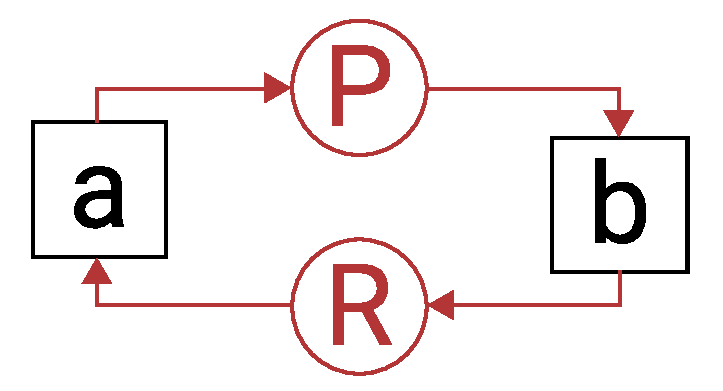
\includegraphics[height=3.75em]{gfx/theory/relationNode.pdf}}}
			\quad\Leftrightarrow\quad
			\exists\ a, b:\ {\color{rot}P(a, b) \land R(b, a)} \numberthis
		\end{align*}
	\item \textbf{Negationskontexte (\textit{negation contexts} oder \textit{cuts}):}
		Für die Negation von Aussagen werden in Konzeptgraphen sog.~Kontexte verwendet.
		Sie lassen sich neben der Negation auch zur Modellierung anderer Zusammenhänge nutzen, diese werden hier allerdings ausgelassen, um den Vergleich mit der Prädikatenlogik zu ermöglichen.
		\begin{align*}
			\vcenter{\hbox{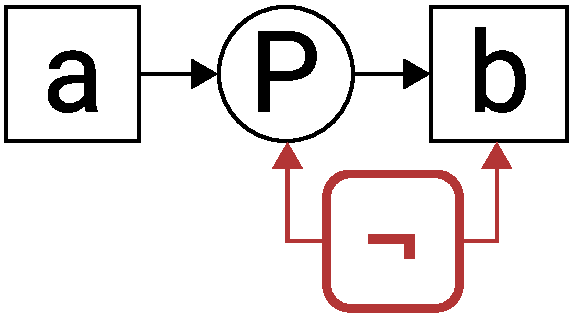
\includegraphics[height=3em]{gfx/theory/negationNode1.pdf}}}
			\quad\Leftrightarrow\quad
			&\exists\ a\ {\color{rot}\lnot\exists}\ b: P(a, b) \numberthis \\
			\quad\Leftrightarrow\quad
			&\exists\ a\ {\color{rot}\forall}\ b: {\color{rot}\lnot} P(a, b)
		\end{align*}
		Die Darstellung von Kontexten mit Knoten und Kanten wird schnell unübersichtlich, daher werden stattdessen Boxen verwendet, die die Kindknoten umschließen.
		\begin{align*}
			\vcenter{\hbox{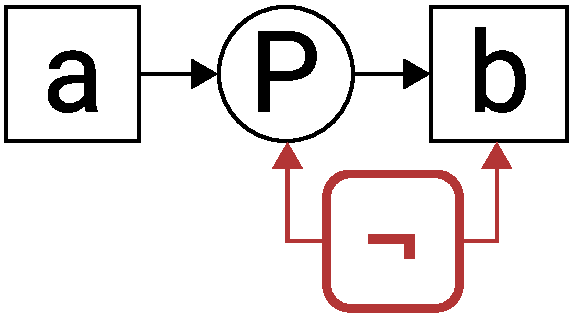
\includegraphics[height=3em]{gfx/theory/negationNode1.pdf}}}
			\quad\Leftrightarrow\quad
			\vcenter{\hbox{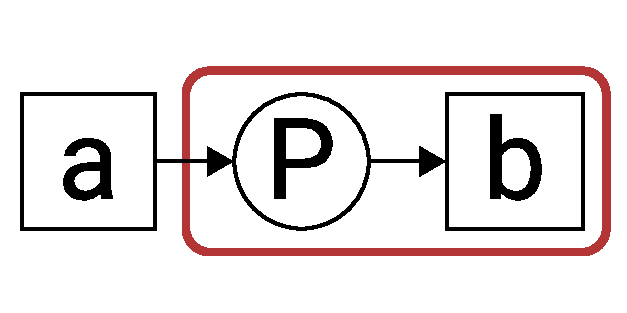
\includegraphics[height=3em]{gfx/theory/negationNode2.pdf}}}
		\end{align*}
		Kontexte können nicht nur Konzeptknoten und Relationsknoten enthalten, sondern auch andere Kontexte.
		Hierbei ist zu beachten, dass alle Knoten und Kontexte höchstens einen Elternkontext haben können;
		die Linien zweier Kontextboxen dürfen sich also nicht schneiden.
		\begin{align*}
			\vcenter{\hbox{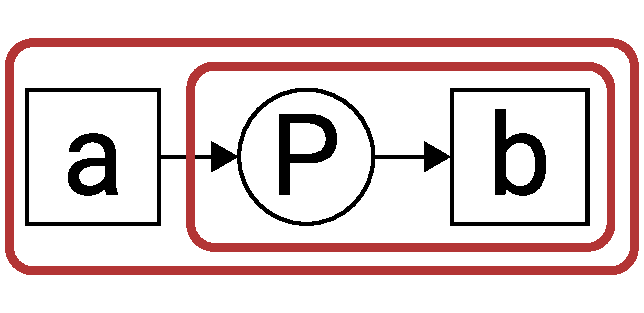
\includegraphics[height=3em]{gfx/theory/negationNode3.pdf}}}
			\quad\Leftrightarrow\quad
			&{\color{rot}\lnot\exists}\ a\ {\color{rot}\lnot\exists}\ b: P(a, b) \numberthis \\
			\quad\Leftrightarrow\quad
			&{\color{rot}\forall}\ a\ \exists\ b: P(a, b)
		\end{align*}
		\begin{align*}
			\vcenter{\hbox{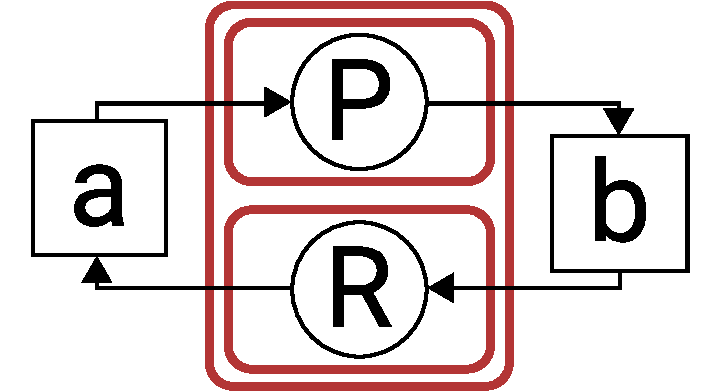
\includegraphics[height=3.75em]{gfx/theory/negationNode4.pdf}}}
			\quad\Leftrightarrow\quad
			&\exists\ a, b: {\color{rot}\lnot}({\color{rot}\lnot} P(a, b) \land {\color{rot}\lnot} R(b, a)) \numberthis \\
			\quad\Leftrightarrow\quad
			&\exists\ a, b: P(a, b)\ {\color{rot}\lor}\ R(b, a)
		\end{align*}
	\item \textbf{Koreferenzkanten (\textit{coreference links}):}
		Entspricht der Äquivalenzrelation.
		\begin{align}
			\vcenter{\hbox{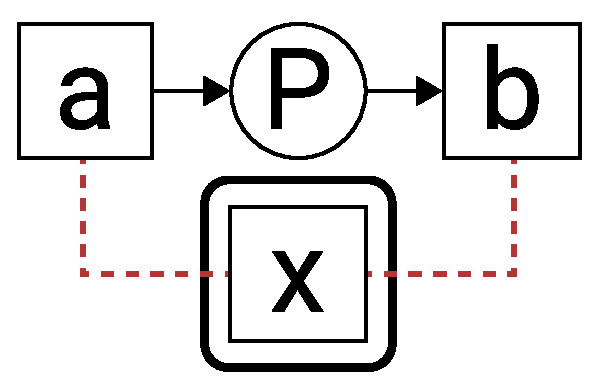
\includegraphics[height=3.75em]{gfx/theory/coreferenceEdge.pdf}}}
			\quad\Leftrightarrow\quad
			&\exists\ a, b: P(a, b) \land \lnot\exists\ x: {\color{rot}a = x \land x = b} \\
			\quad\Leftrightarrow\quad
			&\exists\ a, b: P(a, b) \land {\color{rot}a \neq b} \nonumber
		\end{align}
		Prinzipiell ließe sich die Äquivalenz auch durch Relationsknoten ausdrücken.
		Um syntaktisch zu kennzeichnen, dass es sich nicht um eine beliebige Relation, sondern um eine Äquivalenzrelation handelt, wird dies jedoch i.~d.~R. nicht getan.
		Koreferenzkanten können also als eine Kurzschreibweise verstanden werden, die den Zweck hat die für die Inferenz relevanten Symmetrie-, Transitivitäts- und Reflexivitätseigenschaften zu kennzeichnen.
		\begin{align*}
			\vcenter{\hbox{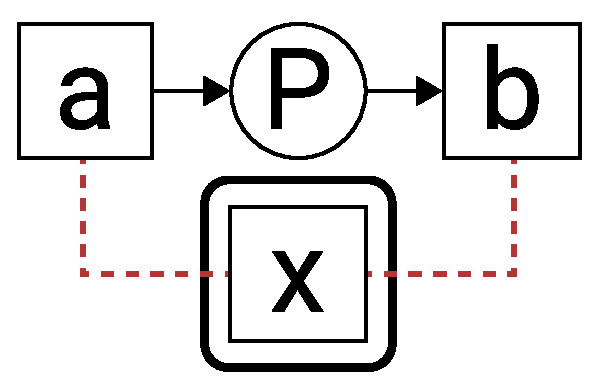
\includegraphics[height=3.75em]{gfx/theory/coreferenceEdge.pdf}}}
			\quad\Leftrightarrow\quad
			\vcenter{\hbox{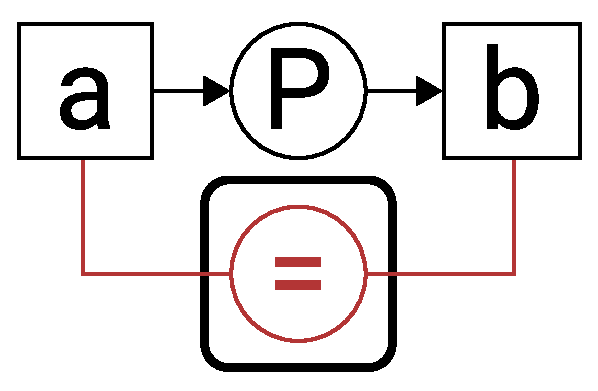
\includegraphics[height=3.75em]{gfx/theory/coreferenceEdgeAlternative.pdf}}}
		\end{align*}
\end{itemize}

\subsection{Dominierende Knoten}%
\label{sec:theory:cg:domnodes}

So wie die Syntaxelemente prädikatenlogischer Ausdrücke nicht beliebig kombiniert werden können, unterliegen auch Konzeptgraphen gewissen Einschränkungen.
Die Einschränkung, dass alle Knoten und Kontexte höchstens einen Elternkontext haben dürfen, wurde bereits erwähnt.
Die zweite wichtige Einschränkung ist das Verbot nicht dominierender Knoten (\textit{dominating nodes}).
Was genau dies bedeutet, wird im Folgenden erläutert. Zuerst müssen Konzeptgraphen jedoch formal spezifiziert werden.
\begin{align*}
	G :=\ &(V, E) \text{, mit globalem Kontext } \top \in V \\
	concept(v) :\Leftrightarrow\ &\text{$v \in V$ ist ein Konzeptknoten} \\
	relation(v) :\Leftrightarrow\ &\text{$v \in V$ ist ein Relationsknoten} \\
	context(v) :\Leftrightarrow\ &\text{$v \in V$ ist ein Kontext, es gilt $context(\top)$} \\
	neg(v) :\Leftrightarrow\ &\text{$v \in V$ ist ein Negationskontext} \displaybreak[0]\\
	nest(c, v) :\Leftrightarrow\ &context(c) \land (c, v) \in E \\
	coref(v_1, v_2) :\Leftrightarrow\ &concept(v_1) \land concept(v_2) \land (v_1, v_2) \in E \\
	arg(r, v) :\Leftrightarrow\ &relation(r) \land concept(v) \land ((r, v) \in E \lor (v, r) \in E) \\ % chktex 35
	E \supseteq\ &\{ (\top, v): v \in V \land \lnot\exists\ c \in V: nest(c, v) \} \displaybreak[0]\\
	a \leq b :\Leftrightarrow\ & (\exists\ x \in V: a \leq x \land x \leq b) \numberthis \\
	& \lor nest(b, a) \lor (\exists\ c \in V: nest(c, a) \land nest(c, b))
\end{align*}
Um die nachfolgenden Definitionen einfacher zu machen, wird der globale Kontext $\top$ eingeführt, der, in Anlehnung an Peirce, \textit{sheet of assertion} genannt wird.
$\top$ enthält alle Knoten, die keinen explizit dargestellten Elternkontext haben.
Die Kontextbox von $\top$ umschließt also den gesamten Konzeptgraphen.
$\leq$ ist eine Quasiordnung und bildet die \textit{enthalten-in}-Relation zwischen Knoten ab, d.~h.\ $a \leq b$ gdw.\ $a$ innerhalb der Box des Elternkontextes von $b$ liegt.
Das größte Element gemäß $\leq$ ist also immer $\top$.
\begin{figure}[h]
	\centering
	\[\vcenter{\hbox{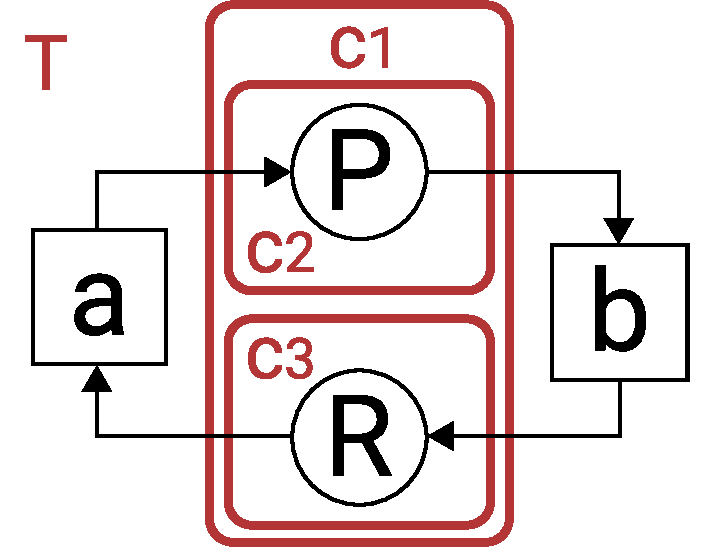
\includegraphics[height=5.25em]{gfx/theory/contextTreeExample1.pdf}}}
	\qquad
	\vcenter{\hbox{
		\begin{tikzpicture}[
			grow=down,
			sloped,
			level distance=2em,
			sibling distance=3em,
			edge from parent/.style={draw=black!70,latex-}]
			\node {\color{rot}$\top$}
				child {
					node (a) {$a$}
				}
				child {
					node (c1) {\color{rot}$c_1$}
						child {
							node (c2) {\color{rot}$c_2$}
								child {
									node {$P$}
								}
						}
						child {
							node (c3) {\color{rot}$c_3$}
								child {
									node {$R$}
								}
						}
				}
				child {
					node (b) {$b$}
				};
				\draw[latex-latex] (a) -- (c1);
				\draw[latex-latex] (c1) -- (b);
				\draw[latex-latex] (c2) -- (c3);
		\end{tikzpicture}
	}}\]
	\caption{Zusammenhang zwischen Kontexten und der $\leq$-Ordnung. Die Existenz eines Pfades von $x$ nach $y$ im obigen baumartigen Graphen, entspricht $x \leq y$.}\label{fig:theory:kgorder}
\end{figure}

Auf Basis von $\leq$ lässt sich nun das Konzept dominierender Knoten definieren.
\begin{align*}
	dom(G) :\Leftrightarrow\ & \forall\ r, v \in V: arg(r, v) \rightarrow r \leq v \numberthis \\ % chktex 35
	& \land \forall\ v_1, v_2 \in V: coref(v_1, v_2) \rightarrow (v_1 \leq v_2 \lor v_2 \leq v_1)
\end{align*}
Für jeden Konzeptgraphen $G$ muss $dom(G)$ gelten.
Eine Intuition für diese Einschränkung ist, dass es nicht sinnvoll ist die Existenz eines Atoms auszudrücken, welches durch nicht existente Variablen parametrisiert ist.
Eine detaillierte Untersuchung des Zwecks dominierender Knoten und eine Beschreibung der entstehenden Probleme, wenn auf die Notwendigkeit dominierender Knoten verzichtet wird, findet sich in~\cite[Abschnitt~14.3]{Dau2003}.
\begin{figure}[h]
	\begin{align*}
		\vcenter{\hbox{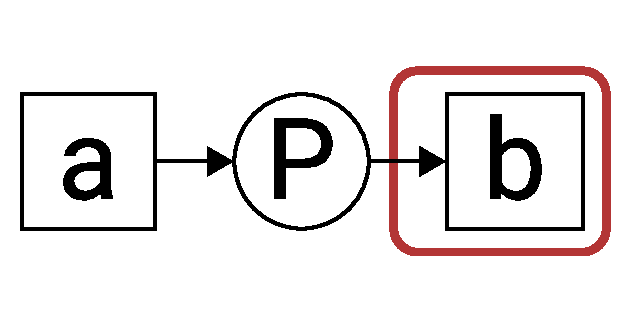
\includegraphics[height=3em]{gfx/theory/dominatingNodeViolation1.pdf}}}
		\quad
		&\text{\color{rot}$\lightning\ \lnot dom(G)$, da $arg(P, b) \land \lnot (P \leq b)$.} \\ % chktex 35
		\vcenter{\hbox{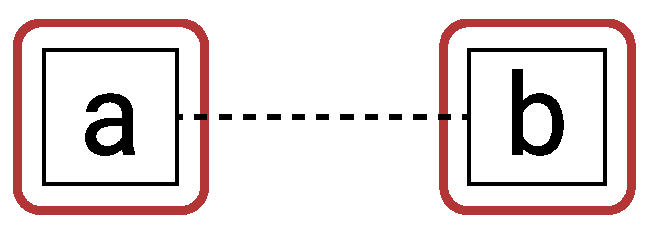
\includegraphics[height=2.25em]{gfx/theory/dominatingNodeViolation2.pdf}}}
		\quad
		&\text{\color{rot}$\lightning\ \lnot dom(G)$, da $coref(a, b) \land \lnot (a \leq b \lor b \leq a)$.}
	\end{align*}
	\caption{Beispiele für fehlerhafte Konzeptgraphen ohne dominierende Knoten.}\label{fig:theory:invalidkg}
\end{figure}

\section{Stanford CoreNLP}%
\label{sec:theory:nlp}

Um natürlichsprachliche Daten in einen Konzeptgraphen zu transformieren, ist im ersten Schritt eine Sprachanalyse notwendig.
Hierfür wurde die Stanford CoreNLP~\cite{CoreNLP} und die Apache OpenNLP~\cite{OpenNLP} Bibliothek in Erwägung gezogen, da beide häufig genutzt, aktiv weiterentwickelt, frei verfügbar und JVM-basiert sind.
Die JVM-Integration ist wichtig, um mit anderen verwendeten Bibliotheken kompatibel zu sein;
mehr hierzu in Abschnitt~\ref{sec:text2kg:implementation}.
Für die Implementation wurde schließlich CoreNLP gewählt, da es mit den mitgelieferten Modellen häufig bessere Ergebnisse als OpenNLP liefert.
Da beide Bibliotheken bzgl.\ ihrer Funktionalität allerdings recht ähnlich sind, kann die NLP Komponente als substituierbar angesehen werden.
Ein Wechsel von CoreNLP auf OpenNLP wäre mit relativ geringem Aufwand möglich.

Im Folgenden wird nun die grundlegende Architektur von CorenNLP beschrieben.
CoreNLP verwendet das in~\ref{sec:related:nlp} vorgestellte Pipeline-Modell.
Die verschiedenen Verarbeitungsstufen der Pipeline werden Annotatoren genannt.
Da die genaue Funktionsweise der Annotatoren ist für diese Arbeit weniger relevant, wichtiger ist ein Überblick über die Art der Ergebnisse, die die Annotatoren liefern.

\paragraph{Tokenization und Lemmatization}
Liefern, wie erwartet, eine Liste von Token bzw.\ eine Liste der Lemmata der Token.
Es werden neben Englisch zahlreiche andere Sprachen und ein Großteil des Unicode Zeichensatzes unterstützt.
Der Tokenizer verwendet zum Finden der Tokens intern einen deterministischen endlichen Automaten.

\paragraph{POS-Tagging}
Ordnet jedem Token eine Wortart und Flexion (POS-Tag) zu.
Die Menge der möglichen POS-Tags wurde aus dem \textit{Penn Treebank Tag Set}~\cite{PennTags} übernommen.
Für das Finden der Tags benutzt CoreNLP sog.\ \textit{Cyclic Dependency Networks}~\cite{Toutanova2003}, eine Erweiterung bayesscher Netze, in denen zyklische Abhängigkeiten erlaubt sind.

\paragraph{Named Entity Recognition (NER)}
Findet sog.\ Entitäten.
CoreNLP benutzt hierfür eine Menge von Entitätsklassen, die sich in drei Kategorien von Klassen unterteilen lässt:
\begin{enumerate}
	\item \textbf{Benannte Entitäten:}
		Person, Ort, Organisation und Sonstige.
		Diese Entitätsklassen werden mittels \textit{Conditional Random Fields}~\cite{Finkel2005}, einer Variante von \textit{Markov Random Fields} (siehe~\ref{sec:theory:psl:mrf}), erkannt.
	\item \textbf{Numerische Entitäten:}
		Geldbetrag, Zahl, Ordinalzahl und Prozentzahl.
		Hierfür wird ein regelbasiertes System verwendet.
		Die so erkannten Token werden zudem normalisiert, um eine leichtere Weiterverarbeitung zu ermöglichen.
	\item \textbf{Temporale Entitäten:}
		Datum, Uhrzeit, Dauer und Menge von Zeitpunkten.
		Diese Klassen werden ebenfalls mit einem regelbasierten System erkannt.
		Mittels SUTime~\cite{Chang2012} werden die erkannten Token anschließend normalisiert und relative Zeitangaben in absolute Zeitpunkte aufgelöst, sofern ein Referenzzeitpunkt gegeben ist.
		Für die Normalisierung wird das TimeML TIMEX3-Format~\cite{TIMEX3} benutzt, mit dem sich auch komplexe Zeitangaben, wie \textit{``twice a week''} (\texttt{type=''set'' value=''P1W'' freq=''2X''}), formal ausdrücken lassen.
\end{enumerate}

\paragraph{Coreference Resolution}
Ermittelt Äquivalenzklassen von Token, die auf das selbe Konzept bzw.\ die selbe Entität verweisen.
CoreNLP stellt hierfür drei verschiedene Systeme bereit:
Ein schnelles, regelbasiertes, deterministisches System, ein etwas langsameres statistisches System und zuletzt ein langsames System, das auf neuronalen Netzen basiert.
Die langsameren Systeme liefern im Schnitt bessere Ergebnisse.

\paragraph{Dependency Parsing}
Dieser Annotator ermittelt die grammatikalischen Beziehungen zwischen Worten.
Das Ergebnis ist ein sog.\ Abhängigkeitsgraph (\textit{Dependency Graph}), in dem die Knoten Token und die Kanten Beziehungen repräsentieren.
CoreNLP verwendet für die Kantentypen \textit{Universal Dependencies Version 2} (UD v2)~\cite{UDv2}, eine Menge von 37 Arten grammatikalischer Beziehungen, die für eine vielzahl natürlicher Sprachen nutzbar ist.
Die Struktur der zurückgegebenen Abhängigkeitsgraphen, basiert auf einem ``\textit{{\color{blau}head}-{\color{rot}modifier}}''-Pattern;
d.~h.\ dass, ausgehend von einem \textit{\color{blau}head}-Token, Kanten zu \textit{\color{rot}modifier}-Token gehen, die die Bedeutug des \textit{\color{blau}heads} verändern.
\[
	\text{\color{rot}Peter's} \xleftarrow{\text{possessive nominal modifier}}
	\text{\color{blau}ball}
	\xrightarrow{\text{adjectival modifier}} \text{\color{rot}red}
\]
Der CoreNLP Dependency Parser nutzt ein sog.\ \textit{Transition-based Parsing}~\cite{Nivre2004}, bei dem alle Token der Reihe nach aus einem Buffer auf einen Stack von aktuell betrachteten Token gelegt werden.
Ein Klassifikator (im Falle von CoreNLP ist dies ein neuronales Netz) wählt dabei in jedem Schritt einen von drei Zustandsübergängen:
\begin{enumerate}
	\item \textbf{LEFT-ARC:}
		Fügt eine Abhängigkeitskante $(i, j)$ vom ersten Token $i$ des Stacks zum zweiten Token $j$ des Stacks ein und entfernt dann $j$ vom Stack.
	\item \textbf{RIGHT-ARC:}
		Fügt eine Abhängigkeitskante $(j, i)$ vom zweiten Token $j$ des Stacks zum ersten Token $i$ des Stacks ein und entfernt dann $i$ vom Stack.
	\item \textbf{SHIFT:}
		Verschiebt das erste Token des Buffers auf den Stack.
\end{enumerate}
Diese drei Zustandsübergänge werden so lange angewandt, bis der Buffer leer ist.
Durch die richtige Kombination von Übergängen lässt sich jeder beliebige Abhängigkeitsgraph beschreiben.

\section{Modellierung von HL-MRFs mit PSL}%
\label{sec:theory:psl}

In~\ref{sec:theory:cg} wurde beschrieben, wie komplexes Wissen durch Konzeptgraphen repräsentiert werden kann;
in~\ref{sec:theory:nlp} wurde beschrieben, wie der Inhalt natürlichsprachlicher Texte extrahiert und durch eine Menge von Abhängigkeiten repräsentiert werden kann.
Dieser Abschnitt beschreibt nun, wie aus einer Menge gegebenener Abhängigkeiten und Fakten neue Abhängigkeiten und Fakten inferiert werden können.
Konkrekt werden hierfür \textit{Hinge-Loss Markov Random Fields} (HL-MRFs) und die \textit{Probabilistic Soft Logic} (PSL) vorgestellt.

\subsection{Markov Random Fields}%
\label{sec:theory:psl:mrf}

MRFs sind, so wie auch bayessche Netze, eine Klasse von \textit{Probabilistischen Graphischen Modellen} (PGM);
d.~h.\ sie sind Graphen, deren Knoten als Zufallsvariablen und deren Kanten als stochastische Abhängigkeiten interpretiert werden.
Im Gegensatz zu bayesschen Netzen, sind die Kanten in MRFs allerdings ungerichtet, es sind also zyklische Abhängigkeiten erlaubt.
Formal beschreibt ein MRF $G$ die multivariate Verteilung $P$ eines Zufallsvektors $X$ gemäß einer Potentialfunktion $\Phi$:
\begin{align*}
	X :=&\ (X_1, \dots, X_n) = \text{Zufallsvektor} \\
	\mathcal{X} :=&\ \text{Menge aller möglichen Werte $(x_1, \dots, x_n)$ von $X$} \\
	G :=&\ (X, E) \\
	\mathcal{C} :=&\ \{ c_1, \dots, c_m \} = \text{Menge der maximalen Cliquen in $G$} \displaybreak[0]\\ % chktex 21
	X_c :=&\ \text{Vektor der Zufallsvariablen in der Clique $c \in \mathcal{C}$} \\
	\Phi_c(x_c) :=&\ \text{Cliquenpotential $\in \mathbb{R}^{+}_0$ der Werte $x_c$ von $X_c$} \\
	P(X = x) =&\ \frac{1}{Z} \prod_{i = 1}^{m} \Phi_{c_i}(x_{c_i}) \text{, mit Normalisierkonst. } Z := \sum_{x \in \mathcal{X}} \prod_{i = 1}^{m} \Phi_{c_i}(x_{c_i}) \numberthis
\end{align*}
Für MRFs gelten drei wichtige Eigenschaften bzgl.\ der Unabhängigkeit der Zufallsvariablen in $X$:
\begin{enumerate}
	\item \textbf{Globale Markov-Eigenschaft:}
		\[
			\forall X_A, X_B, X_S \subseteq X: sep_{X_A, X_B}(X_S) \rightarrow (X_A \perp X_B \mid X_S)
		\]
		Alle Paare $(X_A, X_B)$ von Teilmengen von $X$ sind bedingt unabhängig, sofern die Werte einer separierenden Teilmenge $X_S $ gegeben sind.
		$X_S$ ist separierend ($\Leftrightarrow sep_{X_A, X_B}(X_S)$), wenn alle Pfade von $a \in X_A$ nach $b \in X_B$ einen Knoten $s \in X_S$ enthalten.
	\item \textbf{Lokale Markov-Eigenschaft:}
		\[
			\forall X_i \in X: X_i \perp (X \setminus \Gamma(X_i) \setminus \{X_i\}) \mid \Gamma(X_i)
		\]
		Eine direkte Konsequenz der globalen Markov-Eigenschaft ist die lokale Markov-Eigenschaft.
		Jede Variable $X_i$ ist bedingt unabhängig von ihren nicht benachbarten Variablen, sofern ihre Nachbarschaft $\Gamma(X_i)$ gegeben ist.
	\item \textbf{Paarweise Markov-Eigenschaft:}
		\[
			\forall X_i, X_j \in X: \{X_i, X_j \} \notin E \rightarrow (X_i \perp X_j \mid X \setminus \{ X_i, X_j \})
		\]
		Aus der lokalen Markov-Eigenschaft folgt, dass jedes nicht adjazente Variablenpaar $(X_i, X_j)$ bedingt unabhängig voneinander ist, sofern alle anderen Variablen gegeben sind.
\end{enumerate}

\paragraph{Beispiel}
Die obigen Definitionen sind bislang noch recht abstrakt.
Ein exemplarisches praktisches Einsatzgebiet von MRFs ist das Lösen von SAT-Problemen.
Gegeben sei die SAT-Instanz ${\color{rot}(\lnot A \lor B \lor C)} \land {\color{blau}(\lnot C \lor \lnot D)}$.
MRFs können benutzt werden, um dieses Problem zu modellieren und eine erfüllende Belegung zu finden.\\
\begin{tabular}{m{0.25\textwidth} m{0.75\textwidth}}
	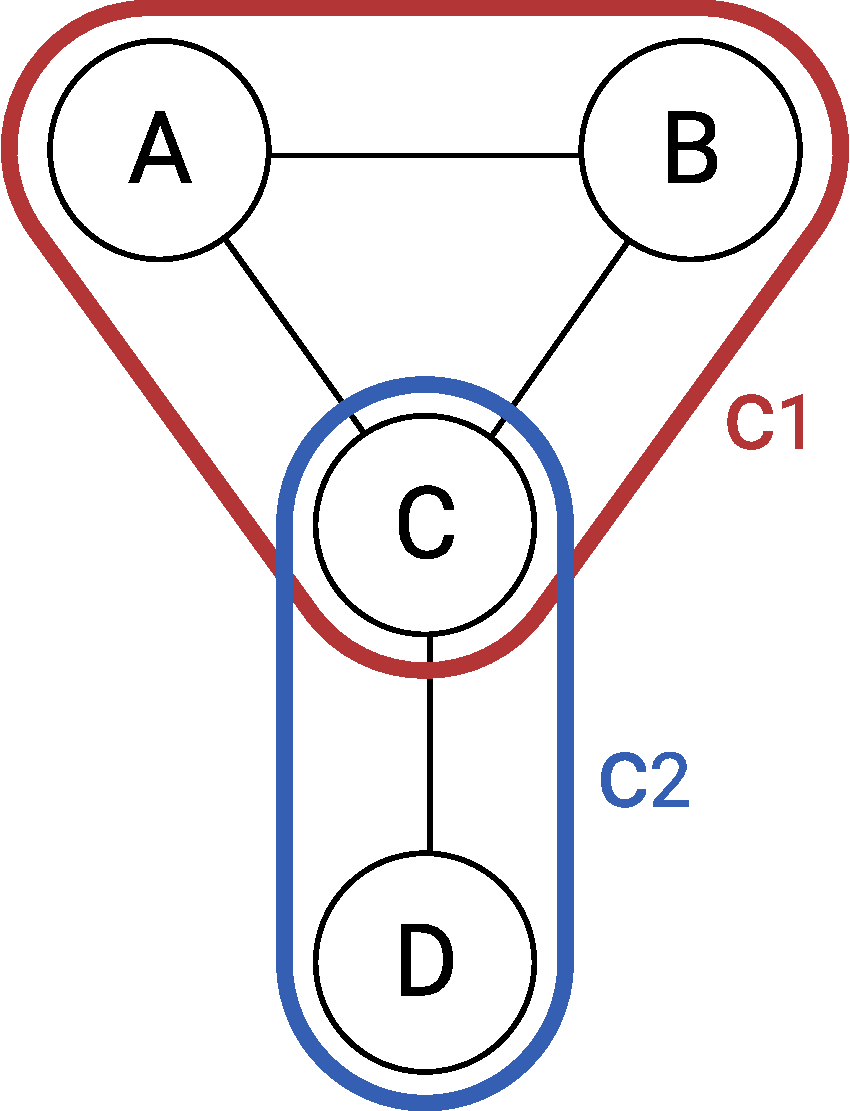
\includegraphics[width=0.23\textwidth]{gfx/theory/mrfExample1.pdf}
	&
	{\begin{align*}
		X :=&\ (A, B, C, D) \text{, mit } Bild(X) = {\{0, 1\}}^4 \\
		\mathcal{C} :=&\ \{{\color{rot}\underbrace{\{ A, B, C \}}_{c_1}}, {\color{blau}\underbrace{\{ C, D \}}_{c_2}}\} \\ % chktex 21
		{\color{rot}\Phi_{c_1}}(a, b, c) :=&\ \min\{ 1 - a + b + c, 1 \} \\ % chktex 21
		{\color{blau}\Phi_{c_2}}(c, d) :=&\ \min\{ 2 - c - d, 1 \} \\ % chktex 21
		P(X = (a, b, c, d)) :=&\ \frac{1}{Z} {\color{rot}\Phi_{c_1}}(a, b, c)\ {\color{blau}\Phi_{c_2}}(c, d)
	\end{align*}}
\end{tabular}\\
Eine Clique repräsentiert in diesem MRF eine Disjunktionsklausel und das Cliquenpotential gibt an, ob eine gegebene Belegung die Klausel erfüllt.
Gemäß dieser Definition, lässt sich die Erfüllbarkeit durch $\max_{x} P(X = x) > 0$ ausdrücken, d.~h.\ die Formel ist erfüllbar, gdw.\ es eine Variablenbelegung mit Eintrittswahrscheinlichkeit~$> 0$ gibt.
Die Normalisierungskonstante $Z$ hat auf das Ergebnis keinen Einfluss und kann daher ignoriert werden.

\paragraph{Das MRF-Inferenzproblem}
Da sich SAT, wie soeben exemplarisch gezeigt, auf MRFs reduzieren lässt, ist das Inferenzproblem, d.~h.\ das Finden einer maximal wahrscheinlichen Belegung der Zufallsvariablen, ein NP-schweres Problem.
Allgemeine, exakte und effiziente Lösungsalgorithmen existieren daher nicht.
Durch Einschränken der Struktur von $G$ und $\Phi$, oder durch das erlauben von Approximationen, lassen sich MRF-Inferenzen jedoch deutlich effizienter finden.
Wenn z.~B. $G$ ein Baum ist, kann mit dem \textit{Belief Propagation} Algorithmus eine exakte Lösung in polynomieller Zeit gefunden werden.

\subsection{Hinge-Loss MRFs}%
\label{sec:theory:psl:hlmrf}

Eine Unterart von MRFs, sind die sog.\ Hinge-Loss MRFs.
Sie sind so strukturiert, dass sich das Inferenzproblem effizient und exakt durch konvexe Optimierungsverfahren lösen lässt.
Es gibt drei wesentliche Unterschiede zu allgemeinen MRFs:
\begin{enumerate}
	\item
		Die Bedeutung von Zufallsvariablen und Kanten zwischen Zufallsvariablen ist klar definiert, da $\Phi$ nicht mehr frei wählbar ist.
		Ähnlich zum Beispiel aus~\ref{sec:theory:psl:mrf}, repräsentieren Zufallsvariablen aussagenlogische Variablen und Cliquen Disjunktionsklauseln.
	\item
		Für den Zufallsvektor $X$ muss $Bild(X) = {[0, 1]}^n$ gelten.
		Diese Einschränkung besteht, da jede HL-MRF-Zufallsvariable als die Wahrscheinlichkeit, dass eine aussagenlogische Variable wahr ist, interpretiert wird.
	\item
		Die Definition der Verteilung $P$ ist etwas anders:
		\begin{align*}
			P(X = x) :=&\ \frac{1}{Z} \prod_{i = 1}^{m} e^{w_i\,\Phi_i(x)} \propto \exp\left(\sum_{i=1}^{m} w_i\,\Phi_i(x)\right) = \exp\left(w\,{\Phi(x)}^\top\right) \numberthis \\
			w :=&\ (w_1, \dots, w_m) \in \mathbb{R}^m,\ \Phi := (\Phi_1, \dots, \Phi_m)
		\end{align*}
		Auf die Cliquenpotentiale $\Phi_i$ wird nun die Exponentialfunktion angewandt, zudem erhalten alle Cliquen bzw.\ Klauseln $c_i$ ein Gewicht $w_i$.
		Das Inferenzproblem $\arg\max_{x} P(X = x)$ ist somit äquivalent zu $\arg\max_{x} w\,{\Phi(x)}^\top$.
\end{enumerate}

\paragraph{KNF-Formel Interpretation}
Aufgrund der Einschränkung von HL-MRFs auf aussagenlogische Ausdrücke, wird im Folgenden die Graphterminologie fallen gelassen und stattdessen die entsprechende aussagen\-logische Terminologie verwendet.
Ein HL-MRF wird nun als Repräsentation einer KNF-Formel $C_1 \land \dots \land C_m$ interpretiert.
Jede Disjunktionsklausel $C_j \in C$ wird durch eine Menge von Variablenindizes positiver Atome $I^{+}_j \subseteq \{1,\dots,n\}$ und eine Menge von Variablenindizes negativer Atome $I^{-}_j \subseteq \{1,\dots,n\}$ beschrieben.
\[
	C_j \cong \left(\bigvee_{i \in I^{+}_j} X_i\right) \lor \left(\bigvee_{i \in I^{-}_j} \lnot X_i\right)
\]

\paragraph{Łukasiewicz Logik}
Da die Variablen der KNF-Formel, gemäß obiger Definition, Werte~$\in [0, 1]$ annehmen können, ist nun noch unklar, wie die Operatoren $\land$, $\lor$ und $\lnot$ funktionieren sollen.
HL-MRFs benutzen hierfür die sog.\ Łukasiewicz Logik aus der Klasse der T-Norm Fuzzy Logiken;
sie ist eine Erweiterung der booleschen Logik, d.~h.\ die Łukasiewicz Operatoren verhalten sich für die Extrema $0$ und $1$ so, wie die booleschen Operatoren, sind aber ebenfalls für alle dazwischen liegenden Eingabewerte definiert.
\begin{align}
	x_1 \land x_2 :=&\ \max\{ x_1 + x_2 - 1, 0 \} \\ % chktex 21
	x_1 \lor x_2 :=&\ \min\{ x_1 + x_2, 1 \} \\ % chktex 21
	\lnot x :=&\ 1 - x
\end{align}
\begin{figure}[h]
	\centering
	\begin{tikzpicture}
		\begin{axis}[
			title={$\land$},
			xlabel=$x_1$,
			ylabel=$x_2$,
			width=0.35\textwidth,
			colormap = {bluered}{color(0cm) = (blau); color(1cm) = (rot)}
		]
			\addplot3[
				mesh,
				samples=12,
				domain=0:1,
				domain y=0:1
			]{max(x + y - 1, 0)};
		\end{axis}
	\end{tikzpicture}
	\begin{tikzpicture}
		\begin{axis}[
			title={$\lor$},
			xlabel=$x_1$,
			ylabel=$x_2$,
			width=0.35\textwidth,
			colormap = {bluered}{color(0cm) = (blau); color(1cm) = (rot)}
		]
			\addplot3[
				mesh,
				samples=12,
				domain=0:1,
				domain y=0:1
			]{min(x + y, 1)};
		\end{axis}
	\end{tikzpicture}
	\begin{tikzpicture}
		\begin{axis}[
			title={$\lnot$},
			xlabel=$x$,
			width=0.35\textwidth,
			colormap = {bluered}{color(0cm) = (blau); color(1cm) = (rot)}
		]
			\addplot[
				surf,
				domain=0:1
			]{1 - x};
		\end{axis}
	\end{tikzpicture}
	\caption{Visualisierung der Łukasiewicz Operatoren $\land$, $\lor$ und $\lnot$.}\label{fig:theory:luklogic}
\end{figure}

Mittels der Łukasiewicz Logik können Disjuktionsklauseln $C_j \in C$ für eine gegebene Variablenbelegung $x$ nun Wahrheitswerte~$\in [0, 1]$ zugeordnet werden.
Dieser Wahrheitswert wird als Klauselpotential $\Phi_j(x)$ verwendet.
Das HL-MRF-Inferenzproblem für KNF-Formeln in Łukasiewicz Logik ist demnach
\begin{alignat*}{3}
	\operatorname*{arg\,max}_{x \in {[0, 1]}^n}& \sum_{C_j \in C} w_j &&\Phi_j(x) \\ % chktex 35
	= \operatorname*{arg\,max}_{x \in {[0, 1]}^n}& \sum_{C_j \in C} w_j &&\left(\left(\bigvee_{i \in I^{+}_j} x_i\right) \lor \left(\bigvee_{i \in I^{-}_j} \lnot x_i\right)\right) \displaybreak[0]\\ % chktex 35
	= \operatorname*{arg\,max}_{x \in {[0, 1]}^n}& \sum_{C_j \in C} w_j \min &&\left\{ \left(\sum_{i \in I^{+}_j} x_i\right) + \left(\sum_{i \in I^{-}_j} (1 - x_i)\right), 1 \right\} \numberthis % chktex 21, chktex 35
\end{alignat*}

Statt die Summe der Wahrheitswerte $\Phi_j(x)$ zu maximieren, kann alternativ auch die Summe der Distanzen zur Erfüllung $\ell_j(x)$, genannt \textit{distance to satisfaction}, minimiert werden;
es gilt $\ell_j(x) = 1 - \Phi_j(x)$.
Gemäß dieser Interpretation ist ein HL-MRF somit eine Menge von gewichteten Constraints $\ell_j(x) \leq 0$, für die eine Lösung mit möglichst wenigen Verletzungen gesucht wird.
Das Inferenzproblem ist also
\begin{align*}
	\operatorname*{arg\,min}_{x \in {[0, 1]}^n}& \sum_{C_j \in C} w_j \max \{ \ell_j(x), 0 \} \displaybreak[0]\\ % chktex 35
	= \operatorname*{arg\,min}_{x \in {[0, 1]}^n}& \sum_{C_j \in C} w_j \max \left\{ 1 - \left(\sum_{i \in I^{+}_j} x_i\right) - \left(\sum_{i \in I^{-}_j} (1 - x_i)\right), 0 \right\} \numberthis % chktex 21, chktex 35
\end{align*}

\begin{figure}[h]
	\centering
	\begin{tikzpicture}
		\begin{axis}[
			xlabel=$x_1$,
			ylabel=$x_2$,
			y dir=reverse,
			width=0.45\textwidth,
			colormap = {bluered}{color(0cm) = (blau); color(1cm) = (rot)}
		]
			\addplot3[
				mesh,
				samples=20,
				domain=0:1,
				domain y=0:1
			]{max(1 - x - y, 0)};
		\end{axis}
	\end{tikzpicture}
	\caption{Visualisierung der Loss-Funktion $\ell_j(x_1, x_2)$ für $C_j \cong X_1 \lor X_2$}\label{fig:theory:hingeloss}
\end{figure}
Wie Abb.~\ref{fig:theory:hingeloss} für den zwei-elementigen Klauselfall veranschaulicht, handelt es sich bei $\ell$ um eine Hinge-Loss Funktion.
Hierher rührt die Bezeichnung Hinge-Loss MRF.\@

\paragraph{MAX-SAT Äquivalenz}
In~\ref{sec:theory:psl:mrf} wurden MRFs anhand des Beispiels der SAT-Instanz ${\color{rot}(\lnot A \lor B \lor C)} \land {\color{blau}(\lnot C \lor \lnot D)}$ veranschaulicht.
Diese KNF-Formel hat folgendes Inferenzproblem, wenn sie als HL-MRF repräsentiert wird:
\[
	\operatorname*{arg\,min}_{(a, b, c, d) \in {[0, 1]}^4} {\color{rot}w_1 \max\{a - b - c, 0\}} + {\color{blau}w_2 \max\{c + d - 1, 0\}} % chktex 21, chktex 35
\]
Da in der Verteilung $P$ von HL-MRFs die Exponentialfunktion auf die Potentiale angewandt wird, bewirkt eine unerfüllte Klausel mit $\Phi_j(x) = 0$ nicht, dass $P(X = x) = 0$.
Stattdessen ist $P(X = x)$ proportional zu der Summe der Wahrheitswerte der Klauseln.
Die HL-MRF-Inferenz beschreibt also nicht SAT, sondern eine Fuzzy-Logik-Entsprechung von MAX-SAT.\@
Ein wichtiger Unterschied zum booleschen MAX-SAT ist, dass Klauseln gewichtet sind;
das Erfüllen einer Klausel mit hohem Gewicht kann das Nicht-Erfüllen mehrerer anderer Klauseln mit niedrigem Gewicht ausgleichen.

\subsection{Probabilistic Soft Logic}%
\label{sec:theory:psl:psl}

Wie soeben beschrieben, sind HL-MRFs ein flexibles Werkzeug, um Probleme, die sich durch MAX-SAT ausdrücken lassen, zu lösen.
Der Schritt von einem konkreten domänenspezifischen Problem in eine Menge von Klauseln $C$ und einen Gewichtsvektor $w$ ist bislang allerdings noch unklar.
An dieser Stelle setzt die \textit{Probabilistic Soft Logic} (PSL) an.
PSL ist eine formale Sprache, um mit einer intuitiven Syntax Klassen von HL-MRFs zu beschreiben.

\subsubsection{Syntax}
Die Syntax von PSL ist an die Prädikatenlogik angelehnt und besteht aus sieben Arten von Elementen:
\begin{enumerate}
	\item \textbf{Konstanten:}
		Repräsentieren konstante Werte, wie z.~B. Strings oder Zahlen.
		Werden für domänenspezifische Daten, wie z.~B. Namen benutzt. \\
		\centerline{\texttt{''Alice'', 32}}
	\item \textbf{Variablen:}
		Werden während einer Inferenz mit Konstanten belegt.
		PSL Variablen sind nicht zu verwechseln mit den Zufallsvariablen in MRFs. \\
		\centerline{\texttt{x, y, z}}
	\item \textbf{Terme:}
		Ein Term ist entweder eine Konstante oder eine Variable.
	\item \textbf{Prädikate:}
		Entsprechen in etwa den prädikatenlogischen Prädikaten.
		Jedes PSL Prädikat hat einen eindeutigen Bezeichner und eine Typsignatur beliebiger Arität.
		Prädikate sind über Konstanten definiert, die Signatur ist daher über den Konstantentypen definiert. \\
		\centerline{\texttt{Person/1: UUID, Name/2: UUID $\times$ String, Age/2: UUID $\times$ Integer}}
	\item \textbf{Atome:}
		Ein Atom ist ein Prädikat der Arität $n$, kombiniert mit einem $n$-Tupel von Termen.
		Das Term-Tupel enthält die Argumente des Prädikates.
		Wenn alle Argumente Konstanten sind, spricht man von einem Grundatom (\textit{ground atom}). \\
		\centerline{\texttt{Person(x), Name(x, ''Alice''), Age(x, 32)}} % chktex 32, chktex 36
	\item \textbf{Literale:}
		Ein Literal ist entweder ein Atom oder ein negiertes Atom. \\
		\centerline{\texttt{Name(x, ''Alice''), !Name(x, ''Bob'')}} % chktex 26, chktex 32, chktex 36
	\item \textbf{Regeln:}
		Eine Regel ist eine gewichtete Disjunktionsklausel von Literalen.
		Die negativen Atome der Klausel bilden dabei den sog.\ Körper $B$ (\textit{body}), die positiven Atome den sog.\ Kopf $H$ (\textit{head}) der Regel.
		Die so zerlegte Disjunktionsklausel lässt sich als Implikationsregel interpretieren:
		\[
			\left(\bigvee_{b \in B} \lnot b\right) \lor \left(\bigvee_{h \in H} h\right) \Leftrightarrow \left(\bigwedge_{b \in B}  b\right) \rightarrow \left(\bigvee_{h \in H} h\right)
		\]
		Mit Implikationen lassen sich nun intuitiv Zusammenhänge zwischen Prädikaten modellieren.\\
		\centerline{\texttt{0.65: Person(x) \& Name(x, ''Alice'') -> Age(x, 32)}} % chktex 26, chktex 32, chktex 36
\end{enumerate}

Die Kombination aus einer Menge von PSL-Regeln und einer Menge von Grundatomen, deren Wahrheitswert bekannt ist, wird PSL-Programm genannt.
